\documentclass[a4paper, 10pt]{article}

\usepackage{tabularx} % extra features for tabular environment
\usepackage{amsmath}  % improve math presentation
\usepackage{graphicx} % takes care of graphic including machinery
\usepackage[margin=1in,letterpaper]{geometry} % decreases margins
\usepackage{cite} % takes care of citations
\usepackage[final]{hyperref} % adds hyper links inside the generated pdf file
\usepackage{ctex}
\usepackage{titlesec}
%\usepackage{CJKutf8, CJK}
\usepackage{makecell}                 % 三线表-竖线
\usepackage{booktabs}                 % 三线表-短细横线
% \usepackage{natbib}
\usepackage{graphicx}				  % 表格单元格逆时针
\usepackage{multirow}				  % 合并单元格
\usepackage{array}
\usepackage{amssymb}				  % 勾
\usepackage{amsmath}
\usepackage{longtable}                % 导入 longtable 宏包,表格自动换行
\usepackage{caption}
\usepackage{subcaption}               % 设置子图
\usepackage{color}					  % 文本颜色包
\usepackage{xcolor}
\usepackage{bbm}					  % 输入指示函数
\usepackage{tablefootnote}			  % 表格注释
\usepackage{pythonhighlight}
\usepackage{fancyhdr}
\usepackage{lastpage}
\usepackage{tocloft}
\pagestyle{fancy}
\fancyhf{}
\fancyhead{}
\fancyfoot{}
\fancyhead[R]{\small Page \thepage\ of \pageref*{LastPage}}
\fancyhead[L]{\small Report}

\usepackage{listings}                 % 导入代码块
\usepackage{xcolor}
\lstset{
	numbers=left, 
	tabsize=1,
	columns=flexible, 
	numberstyle=  \small, 
	keywordstyle= \color{ blue!70},
	commentstyle= \color{red!50!green!50!blue!50}, 
	frame=shadowbox, % 阴影效果
	rulesepcolor= \color{ red!20!green!20!blue!20} ,
	escapeinside=``, % 英文分号中可写入中文
	xleftmargin=2em,
	xrightmargin=2em, 
	aboveskip=1em,
} 

\hypersetup{
	colorlinks=true,       % false: boxed links; true: colored links
	linkcolor=blue,        % color of internal links
	citecolor=blue,        % color of links to bibliography
	filecolor=magenta,     % color of file links
	urlcolor=blue         
}
%++++++++++++++++++++++++++++++++++++++++
\titleformat{\section}{\Large\bfseries\songti}{\thesection}{1em}{}
\titleformat{\subsection}{\large\bfseries\songti}{\thesubsection}{1em}{}
\titleformat{\subsubsection}{\normalsize\bfseries\songti}{\thesubsubsection}{1em}{}
\titleformat{\paragraph}{\small\bfseries\songti}{\paragraph}{1em}{}
\titleformat{\subparagraph}{\footnotesize\bfseries\songti}{\subparagraph}{1em}{}

\begin{document}
	
	
	\title{\songti \zihao{4}2月工作汇报}
	\author{\textrm{Ku Jui}}
	\date{\textrm{Feb 2024}}
	\maketitle
	
	\renewcommand{\figurename}{Figure} % 可以重新定义abstract,因为ctex会覆盖thebibliography
	% 	\begin{abstract}
		%		In this experiment we studied a very important physical effect by measuring the
		%		dependence of a quantity $V$ of the quantity $X$ for two different sample
		%		temperatures.  Our experimental measurements confirmed the quadratic dependence
		%		$V = kX^2$ predicted by Someone's first law. The value of the mystery parameter
		%		$k = 15.4\pm 0.5$~s was extracted from the fit. This value is
		%		not consistent with the theoretically predicted $k_{theory}=17.34$~s. We attribute %this
		%		discrepancy to low efficiency of our $V$-detector.
		%	\end{abstract}
	
	\renewcommand{\tablename}{Table}
	
	% 设置目录标题为居中
	\renewcommand{\cfttoctitlefont}{\hfill\Large\bfseries\songti}
	\renewcommand{\cftaftertoctitle}{\hfill}
	\renewcommand{\contentsname}{Content}
		
	\tableofcontents
	
	\newpage
	
	\part{Pre-Knowledge}	
	
	\section{引言}
		
		低光图像增强(Low-Light Image Enhancement, LLIE)是图像处理领域的一个关键任务,旨在提升低光环境下拍摄图像的视觉质量。该领域的最新进展主要由深度学习技术推动,包括多种学习策略、网络架构、损失函数和训练数据集的应用。低光图像增强在视觉监控、自动驾驶和计算摄影等多个领域具有广泛应用。尤其在智能手机摄影领域,由于相机光圈大小、实时处理需求和存储限制,低光环境下的图像拍摄面临着显著挑战。
		
		%介绍传统的低光图像增强方法
		传统的低光增强方法,如基于直方图均衡化\cite{ji1994adaptive}和Retinex理论\cite{land1965, land1977retinex, jobson1997properties}的方法,虽然能够在一定程度上改善图像质量,但存在一些局限性。直方图均衡化能够提高图像的全局对比度,但可能增加背景噪声的对比度并降低有用图像内容的对比度,导致视觉效果不佳。Retinex算法旨在消除图像照度分量的干扰并还原图像真实色彩,但通常忽略噪声问题,可能导致增强结果中噪声的保留或放大,并且其复杂的优化过程增加了模型的复杂度。
		
		%传统的低光增强方法,如基于直方图均衡\cite{ji1994adaptive}和 Retinex\cite{land1965, land1977retinex, jobson1997properties}的方法,直方图均衡化重新调整图像的直方图分布,一方面增加了图像的全局对比度,另一方面使得亮度在整个图像的分布更加均匀。直方图均衡化的方法非常快速有效,并且是一个可逆操作,但缺点在于其不加选择地处理数据,可能增加背景噪声的对比度,同时降低有用的图像内容的对比度,导致视觉效果欠佳。此外,该方法也无法适用于复杂多变的低光照场景。Retinex 算法的核心思想是消除源图像照度分量干扰,依据反射分量信息还原图像真实色彩。基于 Retinex 的方法能够很大程度改善图像质量,但在应用的过程中仍存在不可忽视的缺点。例如,其通常忽略噪声问题,可能导致增强结果中噪声的保留或放大;有效的先验或正则化的选择具有挑战性,不准确的先验可能导致伪影和颜色偏差;此外,这些方法的复杂优化过程也导致最终的模型较为复杂。
		
		近年来,基于深度学习的低光图像增强技术取得了显著成就,特别是卷积神经网络(CNN)在多个计算机视觉任务中展现出卓越的性能。CNN通过利用注意力机制\cite{yang2021locally,zhang2020attention}和上下文信息,能够从原始图像中有效提取长距离特征\cite{li2018multi, zamir2020learning}。然而,现有的基于CNN的方法在处理局部光照不均匀、颜色信息和细节信息丢失问题时,仍存在过增强或增强不足的挑战,并且增强结果受到感受野大小的限制。
		
		%近年来,基于深度学习的低光图像增强 (LLIE) 方法取得了显著的成功。与传统方法相比,基于深度学习的解决方案在准确性、鲁棒性和速度方面表现更佳,因此受到了越来越多的关注。近年来,基于深度学习的低光图像增强 (LLIE) 技术取得了显著成就,它使用神经网络来学习从弱光图像到自然光图像的映射。与传统方法相比,基于深度学习的解决方案在准确性、鲁棒性和处理速度方面表现更优,因此受到了广泛关注。特别是卷积神经网络(CNN)在多个计算机视觉任务中展现出卓越的性能。CNN 通过利用注意力机制和\cite{yang2021locally, zhang2020attention}上下文信息,能够从原始图像中有效提取多尺度特征\cite{li2018multi, zamir2020learning}。在这些成果的推动下,基于 CNN 的低光图像增强方法得到了持续发展。此外,现有的基于 CNN 的方法大多集中于图像亮度、纹理和颜色的恢复,对于局部光照不均匀、颜色信息和细节信息的丢失问题,仍存在过增强或增强不足的挑战,同时增强结果受到感受野大小的限制,但通过增大卷积核以及多次卷积的方法进行卷积又会增加模型的复杂度。
		
		为了解决这些问题,我们提出了一种新颖的方法(方法名待定)。受到ULite\cite{dinh20231m}中深度可分离卷积的启发,我们将U-Net网络中的卷积改为轴向深度可分离卷积,以减少模型冗余同时保持增强效果。此外,我们借鉴Swin-Unet\cite{cao2022swin}在BottleNeck中使用连续的Swin Transformer块以捕获图像长距离特征,相较于传统的Transformer块,Swin Transformer能够减少参数量和模型复杂度。通过以上改进,我们的方法能够有效提升低光图像的视觉质量,同时保持较低的计算复杂度,具有实际应用的潜力。
		
		%弱光图像增强结果也会受到弱光区域的形状和大小的影响,在深度学习的框架下,卷积神经网络(CNN)通过分层的卷积操作,逐步提取并加工图像的局部特征\cite{jain1991unsupervised, lowe2004distinctive, ojala2002multiresolution},而难以获取图像中的长距离特征,进而导致结果增强过或不足,为了解决这些问题,\textcolor{red}{我们提出了一种方法(方法名待定)}。我们受到ULite\cite{dinh20231m}中深度可分离卷积的启发,将原有的 U-Net 网络中的卷积改为轴向深度可分离卷积,通过这种方式在不损害增强效果的情况下,减少模型冗余。此外,我们借鉴于 Swin-Unet\cite{cao2022swin} 在 BottleNeck 中使用连续的 Swin Transformer 块以捕获图像长距离特征。相较于使用 Transformer 块,使用 Swin Transformer 能够减少参数量和模型复杂度。
		
%		现有的方法仍有很大的改进空间,例如如何在提高亮度的同时消除产生的噪声,如何避免颜色失真现象等。一些现有的方法可以有效地解决一个问题,但往往会忽略了其他问题。不同的方法在不同的数据集上往往具有不同的优势,即在不同的评估标准下有不同的优势,如图.\ref{fig: VE-LOL-L Visual}展示了不同算法在 VE-LOL-L 数据集下的可视化结果。
%
%		\begin{figure}[htbp]
%			\centering
%			\setlength{\abovecaptionskip}{-0.05cm}
%			\begin{subfigure}{0.17\columnwidth}
%				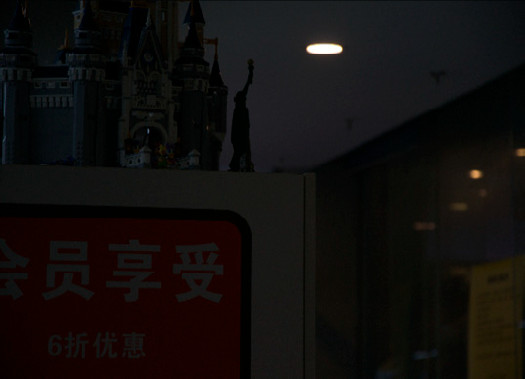
\includegraphics[width=\linewidth]{picture/LLIE/VE-LOL-L/input}
%				\captionsetup{font=scriptsize}
%				\caption*{input \\ \quad }
%				\label{fig: input}
%			\end{subfigure}
%			\begin{subfigure}{0.17\columnwidth}
%				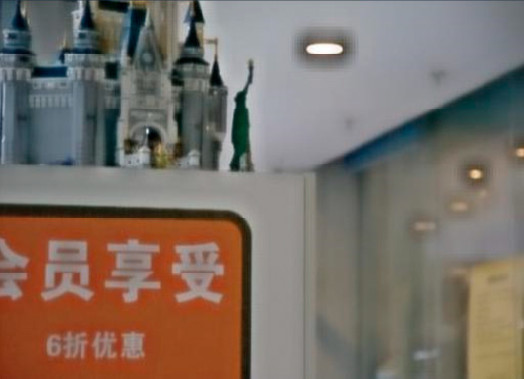
\includegraphics[width=\linewidth]{picture/LLIE/VE-LOL-L/LLNet}
%				\captionsetup{font=scriptsize}
%				\caption*{LLNet \\ (2017)}
%				\label{fig: LLNet_VE_LOL}	
%			\end{subfigure}
%			\begin{subfigure}{0.17\columnwidth}
%				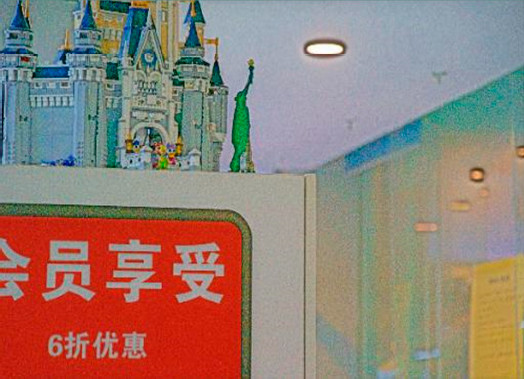
\includegraphics[width=\linewidth]{picture/LLIE/VE-LOL-L/RetinexNet}
%				\captionsetup{font=scriptsize}
%				\caption*{RetinexNet \\ (2018)}
%				\label{fig: RetinexNet_VE_LOL}	
%			\end{subfigure}
%			\begin{subfigure}{0.17\columnwidth}
%				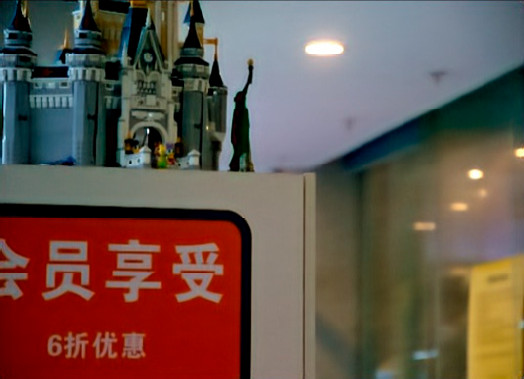
\includegraphics[width=\linewidth]{picture/LLIE/VE-LOL-L/MBLLEN}
%				\captionsetup{font=scriptsize}
%				\caption*{MBLLEN \\ (2018)}
%				\label{fig: MBLLEN_LOL}	
%			\end{subfigure}
%			\begin{subfigure}{0.17\columnwidth}
%				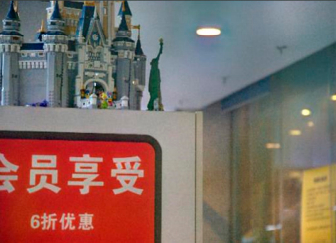
\includegraphics[width=\linewidth]{picture/LLIE/VE-LOL-L/EnlightenGAN}
%				\captionsetup{font=scriptsize}
%				\caption*{EnlightenGAN \\ (2019)}
%				\label{fig: EnlightenGAN_VE_LOL}	
%			\end{subfigure}
%			\begin{subfigure}{0.17\columnwidth}
%				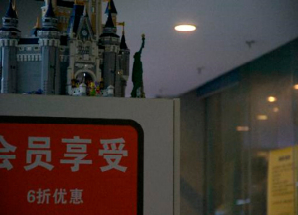
\includegraphics[width=\linewidth]{picture/LLIE/VE-LOL-L/RRDNet}
%				\captionsetup{font=scriptsize}
%				\caption*{RRDNet \\ (2020)}
%				\label{fig: RRDNet_VE_LOL}	
%			\end{subfigure}
%			\begin{subfigure}{0.17\columnwidth}
%				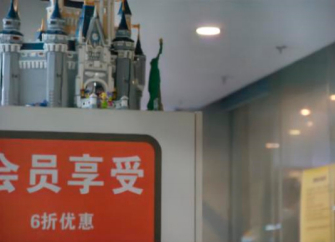
\includegraphics[width=\linewidth]{picture/LLIE/VE-LOL-L/DRBN}
%				\captionsetup{font=scriptsize}
%				\caption*{DRBN \\ (2020)}
%				\label{fig: DRBN_VE_LOL}	
%			\end{subfigure}
%			\begin{subfigure}{0.17\columnwidth}
%				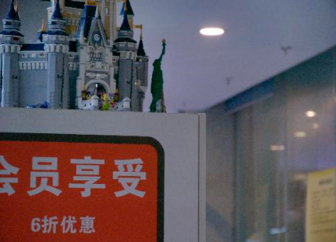
\includegraphics[width=\linewidth]{picture/LLIE/VE-LOL-L/Zero-DCE++}
%				\captionsetup{font=scriptsize}
%				\caption*{Zero-DCE++ \\ (2021)}
%				\label{fig: Zero-DCE++}	
%			\end{subfigure}
%			\begin{subfigure}{0.17\columnwidth}
%				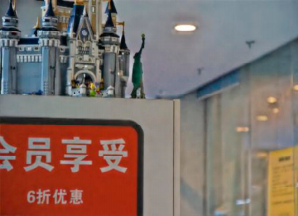
\includegraphics[width=\linewidth]{picture/LLIE/VE-LOL-L/KinD++}
%				\captionsetup{font=scriptsize}
%				\caption*{KinD++ \\ (2021)}
%				\label{fig: KinD++}	
%			\end{subfigure}
%			\begin{subfigure}{0.17\columnwidth}
%				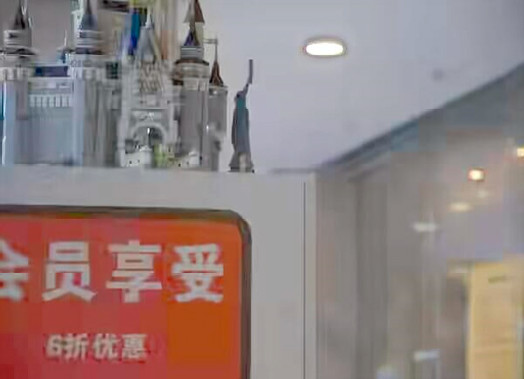
\includegraphics[width=\linewidth]{picture/LLIE/VE-LOL-L/URetinexNet}
%				\captionsetup{font=scriptsize}
%				\caption*{URetinexNet \\ (2022)}
%				\label{fig: URetinexNet}	
%			\end{subfigure}
%			\caption{
%				\label{fig: VE-LOL-L Visual} 
%				不同算法对从VE-LOL-L 数据集采样的低照度图像的可视化结果。
%			}
%		\end{figure}
		
		
		%针对极暗或极亮区域中图像边缘细节恢复的问题,一些研究者提出了在暗区域中加入敏感边缘先验的方法,以降低优化过程中的不适定性,并采用基于编码器-解码器的网络结构和回归损失来执行结构建模。进一步的研究提出了改进的模型,以解决弱光图像中局部边缘失真的问题,并对边缘图与弱恢复图的融合策略进行了优化。
		
		本研究提出了三个主要的创新点:(\textcolor{red}{若并行架构未实现或性能不佳,则可尝试仅通过CNN分支进行图像的弱光恢复,并相应调整创新点,去除并行架构这一创新点。})
		\begin{itemize}
			\item[$\bullet$]
			%首先,提出了一种结合 CNN 和 Transformer 的并行架构用于弱光图像增强。我们发现卷积网络通过合理的增加感受野大小,可以有效捕获图像的局部特征,因而我们利用 UNet 网络对弱光图像进行弱恢复,使用 Swin Transformer 块捕获图像的长距离特征,最后通过特征融合块将二者特征加以融合。
			
			首先,提出了一种结合卷积神经网络(CNN)和Transformer的并行架构用于弱光图像增强。在该架构中,UNet网络用于捕获图像的局部特征并进行初步恢复,而Swin Transformer块用于捕获图像的长距离特征。最后,通过特征融合块将两者的特征进行融合,以实现更全面的图像增强效果。
			\item[$\bullet$] 
			%其次,在CNN分支中,提出了一个深度语义模块,融合 Swin Transformer 分支,能有效捕获图像长距离特征;
			其次,提出了一个深度语义模块,该模块融合了Swin Transformer分支,使CNN分支能够有效捕获图像的长距离特征。这种设计增强了CNN分支的能力,使其能够更好地理解图像的全局上下文信息。
			\item[$\bullet$]
			%最后,我们将深度可分离卷积融合进 CNN 分支中,应用于轻量级网络用于提取图像的局部特征;
			最后,将深度可分离卷积融合进CNN分支中,应用于轻量级网络用于提取图像的局部特征。这种设计旨在减少模型的参数量和计算复杂度,同时保持对局部特征的有效提取能力。
		\end{itemize}
		
		\section{实验计划}

		实验的过程中,确保所有的实验在相同的硬件和软件环境下进行,并且为了确保结果的可靠性,可能需要多次运行实验并取平均值。我们主要基于 PyTorch 进行模型的搭建、训练和评估。基于 scikit-image 库计算 PSNR、SSIM 等评价指标。首先构建 U-Net 基本架构模型,然后实现 Swin Transformer 块中的LocalselfAttention类,PositionEncoding类,PositionEmbedding类。

		\subsubsection{Dataset}
		
		Tab. \ref{tab: Paired_training_datases} 展示了我们在实验中会使用到的弱光数据集,这些数据集包含真实数据与合成数据。对于每个数据集,我们需要进行如下操作:
		
		\begin{itemize}
			\item [$\bullet$]
			预处理: 确保所有图像都经过相同的预处理步骤,如尺寸调整、归一化等。
			
			\item [$\bullet$]
			分割: 将每个数据集分为训练集、验证集和测试集。
		\end{itemize}
		
		\begin{table}[!htbp]
			\centering
			\tiny
			%\resizebox{\textwidth}{!}{ %按照宽度调整调整表格大小
				\begin{tabular}{>{\centering\arraybackslash}m{2.5cm}|c|c|c|c}
					
					\hline
					
					\textbf{Name} & \textbf{Number} & \textbf{Format} & \textbf{Real/Syn} & \textbf{Video} \\
					
					\hline
					
					LOL\cite{wei2018deep} & 500 & RGB & Real & \\
					
					SCIE\cite{cai2018learning} & 4,413 & RGB & Real & \\
					
					VE-LOL-L\cite{jiang2019learning} & 2,500 & RGB & Real+Syn & \\
					
					\hline
					
				\end{tabular}
				%}
			\captionsetup{font=scriptsize} %设置标题字体与表格字体一致
			\caption{\label{tab: Paired_training_datases}
				Summary of paired training datasets. 'Syn' represents Synthetic.} %表格的标题
			
		\end{table}
		
		\subsubsection{Train}
		
		\begin{itemize}
			\item [$\bullet$]
			基线模型: 首先,训练基线模型。
			
			\item [$\bullet$]
			消融研究: 接着,训练正常 BottleNeck 的模型,以进行消融实验。
		\end{itemize}
		
		\subsubsection{Performance Evaluation}
		
		对于每个数据集,使用以下指标评估模型性能:
		
		\begin{itemize}
			\item[$\bullet$]
			峰值信噪比 (PSNR)
			\item[$\bullet$]
			结构相似性指数 (SSIM)
			\item[$\bullet$]
			感知图像质量评估 (LPIPS)
		\end{itemize}
				
		\subsubsection{Loss Function}
		
		\begin{equation}
			J_{Huber}(\delta)= \frac{1}{N}\sum_{i=1}^{N}
			\left\{
			\begin{aligned}
				&\frac{1}{2}{\left\|\hat{y}_i - y_i \right\|}_2^{2}, \left\| \hat{y}_i -y_i \right\| < \delta , \\
				&\delta\left({\left\|\hat{y}_i - y_i \right\|}_1 - \frac{1}{2}\delta \right), \left\| \hat{y}_i -y_i \right\| \geq \delta.
			\end{aligned}
			\right.
			\label{eq: huber loss}
		\end{equation}
		
		\begin{equation}
			\begin{aligned}
				\ell_{feat}^{\phi,j} (\hat{y},y) = \frac{1}{C_{j}H_{j}W_{j}}{\left\| \phi_{j}(\hat{y})-\phi_{j}(y)\right\|}_{2}^2
			\end{aligned}
			\label{eq: perceptual loss}
		\end{equation}
		
		\begin{equation}
			\begin{aligned}
				\mathcal{L}^{\text{SSIM}}(P)=1-\text{SSIM}(\tilde{p}).
			\end{aligned}
			\label{eq: revised_SSIM loss}
		\end{equation}
		
		
		一共尝试以下两种损失函数的搭配方式:
		
		\begin{itemize}
			\item[$\bullet$]
			休伯损失函数和SSIM损失函数
			
			\begin{equation}
				L_{loss} = \alpha J_{Huber}(\delta) + \beta \mathcal{L}^{\text{SSIM}}(P)
			\end{equation}
			
			\item[$\bullet$]
			休伯损失函数,SSIM损失函数,Perceptual损失函数(耗费更多训练时间)
			
			\begin{equation}
				L_{loss} = \alpha J_{Huber}(\delta) + \beta \mathcal{L}^{\text{SSIM}}(P) + \gamma \ell_{feat}^{\phi,j} (\hat{y},y)
			\end{equation}
		\end{itemize}
		
%%%%%%%%%%%%%%%%%%%%%%%%%%%%%%%%%%%%%%%%%%%%%%%%%%%%%%%%%%%%%%%%%%%%%%%%%%%%%%%%%%%%%%%%%%%%%%%%%%%%
%%%%%%%%%%%%%%%%%%%%%%%%%%%%%%%%%%%%%%%%%%%%%%%%%%%%%%%%%%%%%%%%%%%%%%%%%%%%%%%%%%%%%%%%%%%%%%%%%%%%
%%                                                                                                %% 
%%								          Paper reading                                           %%
%%                                                                                                %%
%%%%%%%%%%%%%%%%%%%%%%%%%%%%%%%%%%%%%%%%%%%%%%%%%%%%%%%%%%%%%%%%%%%%%%%%%%%%%%%%%%%%%%%%%%%%%%%%%%%%
%%%%%%%%%%%%%%%%%%%%%%%%%%%%%%%%%%%%%%%%%%%%%%%%%%%%%%%%%%%%%%%%%%%%%%%%%%%%%%%%%%%%%%%%%%%%%%%%%%%%	

	
	\part{Paper Reading}
	
	\section{Lightweight Model}
		
		\subsection{(2023.8)1M parameters are enough? A lightweight CNN-based model for medical image segmentation}
		
		\paragraph{1M的参数就足够了吗?一种基于 CNN 的轻量级医学图像分割模型}
		
		\paragraph{(APSIPA ASC 2023 2区) doi: 10.1109/APSIPAASC58517.2023}
		
			\subsubsection{Research Background}
			
			卷积神经网络 (CNNs) 和基于 Transformer 的模型由于能够提取图像的 High-Level 特征和捕捉图像的重要方面而被广泛应用于医学图像分割。然而,在对高精度的需求和对低计算成本的期望之间往往存在权衡。具有更高参数的模型理论上可以获得更好的性能,但也会导致更高的计算复杂性和更高的内存使用率,因此实现起来并不实用。
			
			在本文中,作者寻找一种轻量级的基于 U-Net 的模型,它可以实现几乎相当甚至更好的性能,即 U-Lite。作者基于深度可分离卷积的原理设计了 U-Lite,这样该模型既可以利用神经网络的强度,又可以减少大量的计算参数。
			
			\subsubsection{Contribution}
			
			具体来说,作者提出了在编码器和解码器中都具有 $7\times7$ 的轴向深度卷积,以扩大模型的感受野。为了进一步提高性能,作者使用了几个具有 $3\times3$ 的轴向空洞深度卷积作为作者的分支之一。
			
			总体而言,U-Lite仅包含 878K 参数,比传统 U-Net 少35倍。与其他最先进的架构相比,所提出的模型降低了大量的计算复杂性,同时在医学分割任务上获得了令人印象深刻的性能。
			
			在本文中,作者重新思考了一种用于医学分割任务的高效轻量级架构,以进一步探索一种能够有效解决这一问题的高性能模型。
			
			简而言之,本文的主要贡献有3个方面:

			\begin{itemize}
				\item[(1)] 基于深度可分离卷积的概念,提出了轴向深度卷积模块的使用方法。该模块帮助模型解决每一个复杂的体系结构问题:扩大模型的感受野,同时减少沉重的计算负担。
				
				\item[(2)] 提出U-Lite,一种基于CNN的轻量级、简单的架构。据作者所知,U-Lite是为数不多的在性能和参数数量方面超过最近高效紧凑型网络UneXt的型号之一。
				
				\item[(3)] 作者已经在医学分割数据集上成功地实现了该模型,并取得了可观的效果。
			\end{itemize}
			
			\subsubsection{Approach}
			
			作者提出的 U-Lite 模型的概述如 Fig. \ref{fig: U-Lite Architecture} 所示。作者遵循 U-Net 的对称编码器-解码器架构,并以一种有效的方式设计U-Lite,以便该模型能够利用 CNN 的强度,同时保持计算参数的数量尽可能少。
			
			\begin{figure}[htbp]
				% read manual to see what [ht] means and for other possible options
				\centering 
				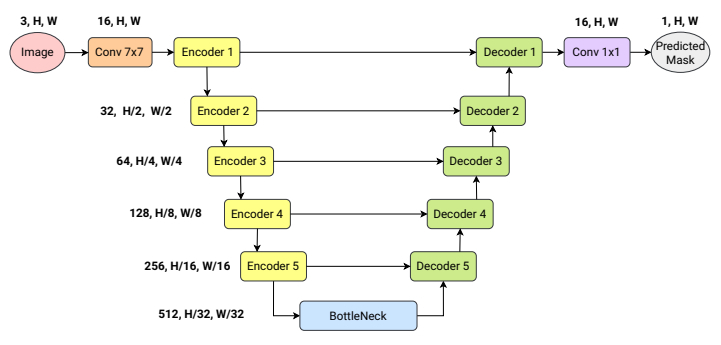
\includegraphics[width=\columnwidth]{picture/Lightweight Model/U-Lite Architecture}
				%\captionsetup{font=scriptsize}
				\caption{
					\label{fig: U-Lite Architecture} 
					The proposed U-Lite architecture.
				}
			\end{figure}
			
			为此,作者深思熟虑地提出了一个轴向深度卷积模块,如 Fig. \ref {fig: Axial Depthwise Convolution module} 所示。描述 U-Lite 的操作,形状为 $\left(3, H, W\right)$ 的输入图像通过 $3$ 个阶段被馈送到网络:编码器阶段、Bottleneck阶段和解码器阶段。U-Lite遵循分层结构,其中编码器提取形状$\left(C_i, \frac{H}{2^{i}}, \frac{W}{2^i}\right)$中的 $6$ 个不同 Level 的特征,其中 $i \in \{0,1,2, \ldots ,5\}$。
			
			\begin{figure}[htbp]
				% read manual to see what [ht] means and for other possible options
				\centering 
				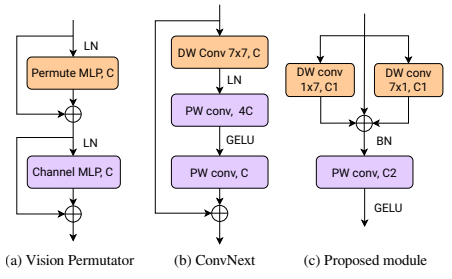
\includegraphics[width=0.6\columnwidth]{picture/Lightweight Model/Axial Depthwise Convolution module}
				%\captionsetup{font=scriptsize}
				\caption{
					\label{fig: Axial Depthwise Convolution module} 
					Architectures of (a) Vision Permutator, (b) ConvNext, and (c) Proposed Axial DW Convolution module. The proposed module is inspired by Vision Permutator’s and ConvNext's designs.
				}
			\end{figure}
			
			Bottleneck 和解码器参与处理这些特征,并将它们放大到原始形状以获得分割 Mask。作者还在编码器和解码器之间使用 skip connections 连接。值得注意力的是,尽管 U-Lite 的设计很简单,但由于轴向深度卷积模块的贡献,该模型在分割任务上仍然表现良好。
			
			\paragraph{Axial Depthwise Separable Convolution Module}

			轴线深度可分离卷积是一种特殊的卷积操作,它将传统的深度可分离卷积进一步分解为两个独立的轴向卷积:水平轴向卷积和垂直轴向卷积。
			
			\begin{itemize}
				\item[(1)]
				\textbf{深度可分离卷积 (Depthwise Separable Convolution):} 这是一种将标准卷积分解为两个较小的卷积操作的技术。首先是深度卷积(Depthwise Convolution),它对每个输入通道单独应用卷积核,然后是逐点卷积(Pointwise Convolution),它使用 1x1 的卷积核将深度卷积的结果合并在一起。这种分解减少了计算量和参数数量。
				\item[(2)]
				\textbf{轴向卷积 (Axial Convolution):} 在轴向深度可分离卷积中,深度卷积被进一步分解为两个轴向操作:一个沿水平方向(宽度),另一个沿垂直方向(高度)。这样做可以进一步减少计算量,同时保持良好的特征提取能力。
			\end{itemize}
			
			视觉 Transformer 的成功推动了研究和改进这种特殊结构的各种工作。Swin-Transformer 通过将自注意力计算限制在大小为 $7 \times 7$ 的非重叠局部窗口,降低了 Transformer 的计算复杂性。ConvNext 实现了这一修改,并在 CNN 架构中采用了 kernel 大小为 $7 \times 7$ 的卷积,使 ResNet 在 ImageNet 上的最高精度达到 $86.4\%$。
			
			Vision Permutator 利用线性投影来沿着高度和宽度维度分别编码特征表示。
			
			\textbf{论文提及:如果用局部感受野\footnote{局部感受野(Local Receptive Field)指的是一个神经元只对输入数据的一个局部区域进行响应,这有助于捕捉图像中的局部特征,如边缘、角点等。}取代ViT的十字形感受野\footnote{十字形感受野(Cross-shaped Receptive Field)指的是在ViT中,每个注意力头计算的是全局的自注意力,这意味着每个输出位置的注意力是基于整个输入图像的。但在一些变体中,例如CrossViT,会使用十字形的感受野,即在水平和垂直方向上分别计算注意力,以减少计算量并捕捉不同方向的特征。},就像 Swin Transformer\footnote{Swin Transformer 利用局部感受野取代十字感受野,它将输入图像划分为多个小块,然后在这些小块内部计算自注意力,从而实现局部感受野。其可以减少计算量,增强模型的泛化能力,并提高效率。} 对 ViT 所作的那样,会发生什么?}
			
			感受野是一个视觉模型效果的至关重要的属性之一,因为模型是无法建模它感知不到的区域的。在 DeepLab 系列算法中,空洞卷积在不增加参数量的同时可以快速增大感受野。Swin-Transformer\cite{liu2021swin} 仅仅通过移动窗口的方式来增加感受野的方式在增加感受野上仍然过于缓慢,因为这个算法仍然需要大量堆叠网络块的形式来增加感受野。CSwin-Transformer(Cross-shape window)\cite{dong2022cswin} 是 swin-Transformer 的改进版,它提出了通过十字形的窗口来进行自注意力计算,它不仅计算效率非常高,而且能够通过两层计算就获得全局的感受野。
			
			因此,作者提出了轴向深度卷积模块,作为 Vision Permutator 和卷积设计的组合。该算子的数学公式表示为
			
			\begin{equation}
				\begin{aligned}
					x^\prime = x + \text{DW}_{1 \times n}(x) + \text{DW}_{n \time 1}(x) \\
					y = \text{GELU}\left(PW_{C_1 \rightarrow C_2} \left(\text{BN}\left(x^\prime \right)\right)\right)
				\end{aligned}
				\label{eq: Axial Depthwise Convolution module}
			\end{equation}
			
			\begin{figure}[htbp]
				% read manual to see what [ht] means and for other possible options
				\centering 
				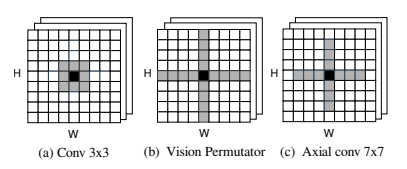
\includegraphics[width=0.6\columnwidth]{picture/Lightweight Model/Receptive Field}
				%\captionsetup{font=scriptsize}
				\caption{
					\label{fig: Receptive Field} 
					The receptive field comparison between Convolution $3 \times 3$,
					Vision Permutator, and Axial convolution $7 \times 7$. Axial convolution
					$7 \times 7$ offers a large receptive field compared with Convolution
					$3 \times 3$ while using fewer computational parameters than Vision
					Permutator.
				}
			\end{figure}
			
			其中,$x$为输入特征,$y$为输出特征;DW、PW和BN分别代表深度卷积、点卷积和批量归一化,$1 \times n$和$n \times 1$是卷积的 kernel 大小;$C_1$ 和 $C_2$ 表示特征图的输入和输出通道的数量。在作者的实验中,$n=7$。为了实现最小和灵活的设计,作者使用了一种独特的逐点卷积,而不添加残差连接,允许自适应地改变输入通道的数量。
			
			\paragraph{Encoder Block and Decoder Block}
			
			编码器和解码器块的设计原理如下:
			
			\begin{itemize}
				\item [(1)] 遵循深度可分离卷积架构。这是从头开始成功构建轻量级模型的重要关键。深度可分离卷积在使用较少参数的同时,提供了与传统卷积相同的性能,从而降低了计算复杂性,使模型更加紧凑。
				\item [(2)] 限制使用不必要的操作op。只需使用普通的MaxPooling和UpSampling层。不需要诸如转置卷积之类的高参数消耗算子。逐点卷积算子可以同时扮演两个角色:沿着特征图的深度对特征进行编码,同时灵活地改变输入通道的数量。
				\item [(3)] 每个编码器或解码器块采用一个批量标准化层,并以GELU激活功能结束。作者对批处理规范化和层规范化进行了性能比较,但没有太大区别。应用GELU是因为与ReLU和ELU相比,在使用GELU时证明了其在准确性方面的改进。
			\end{itemize}
			
			U-Lite的编码器和解码器结构如 Fig. \ref{fig: Encoder and Decoder} 所示。
			
			\begin{figure}[htbp]
				% read manual to see what [ht] means and for other possible options
				\centering 
				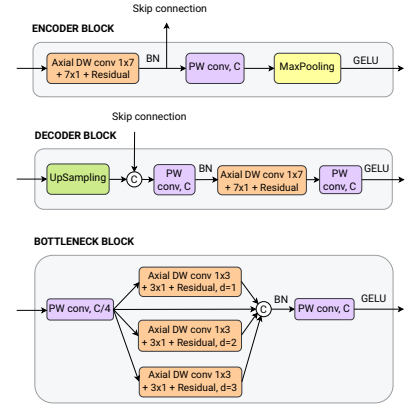
\includegraphics[width=0.6\columnwidth]{picture/Lightweight Model/Encoder and Decoder}
				%\captionsetup{font=scriptsize}
				\caption{
					\label{fig: Encoder and Decoder} 
					Encoder, decoder, and bottleneck blocks. Designed based on Depthwise Separable Convolution concept. Each block adopts one Batch Normalization layer and ends with a GELU activation function.
				}
			\end{figure}
			
			\paragraph{Bottleneck Block}
			
			为了进一步提高U-Lite的性能,作者将kernel大小 $n=3$ 的轴向扩展深度卷积应用于 Bottleneck 块。应用的空洞率为 $d = 1,2,3$。作者使用具有大小为3的 kernel 的轴向扩张卷积,原因有两个:
			
			\begin{itemize}
				\item [(1)] 大小为3大小的kernel更适合底层特征的空间形状,其中这些特征的高度和宽度减少了多次。
				
				\item [(2)] 当使用具有不同空洞率的空洞卷积来捕获后面阶段的High-Level特征的多空间表示时,它给出了更好的性能。
			\end{itemize}
			
			为了进一步减少可学习参数的数量,在 Bottleneck 块的开头采用了逐点卷积层。这有助于在将最后一层特征提供给轴向扩展深度卷积机制之前缩小其通道尺寸。
			
			\subsubsection{Future}
		
			-
	\section{Edge Detection}
		
		\subsection{(2022.3)Survey of Image Edge Detection}
			
		\paragraph{图像边缘检测综述}
			
		\paragraph{(Frontiers in Signal Processing 2区) doi: 10.3389/frsip.2022.826967}
			
			\subsubsection{Research Background}
				
			作者对边缘检测算法进行全面的分析和专题研究。首先,通过对传统边缘检测算法的多层次结构进行分类,介绍了各类算法的原理和方法。其次,重点分析了重点分析了基于深度学习的边缘检测算法,分析了各算法的技术难点、方法优势以及骨干网络选择。然后,通过在BSDS500和NYUD数据集上的实验,进一步评估了每种算法的性能。可以看出,目前的边缘检测算法的性能已经接近甚至超越了人类视觉水平。目前,关于图像边缘检测的综合综述文章较少。本文致力于对边缘检测技术进行全面的分析,旨在为相关人员轻松跟进边缘检测的最新发展并做出进一步的改进和创新提供参考和指导。
			
			\subsubsection{Contribution}
			
			由于图像边缘的重要性,图像边缘检测自提出以来就受到了研究人员的广泛关注,Fig. \ref{fig: Development} 说明了边缘检测算法的发展。
			
			\begin{figure}[htbp]
				% read manual to see what [ht] means and for other possible options
				\centering 
				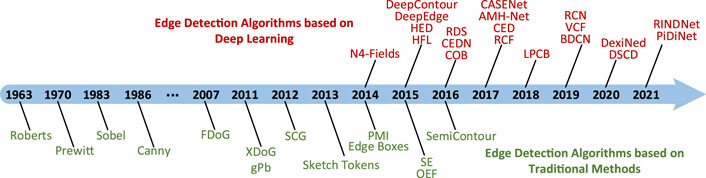
\includegraphics[width=\columnwidth]{picture/Edge Detection/Development}
				%\captionsetup{font=scriptsize}
				\caption{
					\label{fig: Development} 
					Development of edge detection algorithms based on traditional and deep learning methods.
				}
			\end{figure}
			
			随着深度学习的不断发展,出现了各种基于 CNN 实现边缘检测的方法。2015 年,Bertasius 等人。改变了传统的自下而上的边缘检测思路,提出了一种自上而下的多尺度发散深度网络 DeepEdge \cite{bertasius2015high} 用于边缘检测。同年,Xie等人开发了整体嵌套边缘检测算法HED\cite{xie2015holistically},解决了基于图像的整体训练和预测以及多尺度多层次特征学习的问题。 2017年,Liu等人,提出了一种使用更丰富的卷积特征的精确边缘检测器RCF\cite{liu2017richer}。 2019年,Deng等人,提出了一种新颖的端到端边缘检测系统DSCD\cite{deng2020deep},它有效地利用多尺度和多层次特征来产生高质量的物体边缘输出。 2021年Su等人,设计了 PiDiNet\cite{su2021pixel},一种简单、轻量级且高效的边缘检测架构。
			
			作者通过在 BSDS500 和 NYUD 数据集上的实验,进一步评价了上述每种算法的性能。
			
			\begin{table}[!htbp]
				\centering
				\tiny
				%\resizebox{\textwidth}{!}{ %按照宽度调整调整表格大小
					\begin{tabular}{c|c|c|c|c|c|c|c|c|c}
						
						\hline
						
						\textbf{} & \textbf{Canny} & \textbf{FDoG} & \textbf{XDoG} & \textbf{gPb} & \textbf{SCG} &  \textbf{Sketch tokens} & \textbf{SE} & \textbf{OEF} & \textbf{SemiContour} \\
						
						\hline
						
						ODS$\uparrow$ & 0.60 & 0.63 & 0.65 & 0.71 & 0.72 & 0.73 & 0.75 & \textbf{0.76} & 0.74 \\
						
						OIS$\uparrow$ & 0.63 & 0.65 & 0.66 & 0.74 & 0.74 & 0.75 & 0.77 & \textbf{0.79} & 0.77 \\
						
						\hline
						
					\end{tabular}
					%}
				\captionsetup{font=scriptsize} 
				\caption{\label{tab: Algorithms on the BSDS500 dataset}
					Performance comparison of conventional edge detection based algorithms on the BSDS500 dataset.} 
			\end{table}
			
			\begin{table}[!htbp]
				\centering
				\tiny
				%\resizebox{\textwidth}{!}{ %按照宽度调整调整表格大小
					\begin{tabular}{c|c|c|c|c|c|c|c|c|c}
						
						\hline
						
						\textbf{} & \textbf{Canny} & \textbf{FDoG} & \textbf{XDoG} & \textbf{gPb} & \textbf{SCG} &  \textbf{Sketch tokens} & \textbf{SE} & \textbf{OEF} & \textbf{SemiContour} \\
						
						\hline
						
						ODS$\uparrow$ & 0.47 & 0.49 & 0.50 & 0.53 & 0.62 & 0.63 & 0.65 & \textbf{0.69} & 0.68 \\
						
						OIS$\uparrow$ & 0.46 & 0.50 & 0.51 & 0.54 & 0.63 & 0.63 & 0.67 & 0.69 & \textbf{0.70} \\
						
						\hline
						
					\end{tabular}
					%}
				\captionsetup{font=scriptsize} 
				\caption{\label{tab: Algorithms on the NYUD dataset}
					Performance comparison of conventional edge detection based algorithms on the NYUD dataset.} 
			\end{table}
			
			\begin{table}[!htbp]
				\centering
				\tiny
				%\resizebox{\textwidth}{!}{ %按照宽度调整调整表格大小
					\begin{tabular}{c|c|c|c|c|c|c|c|c|c}
						
						\hline
						
						\textbf{} & \textbf{N4-fields} & \textbf{DeepEdge} & \textbf{HED} & \textbf{HFL} & \textbf{CEDN} &  \textbf{RDS} & \textbf{COB} & \textbf{CASENet} & \textbf{RCF} \\
						
						\hline
						
						ODS$\uparrow$ & 0.47 & 0.49 & 0.50 & 0.53 & 0.62 & 0.63 & 0.65 & \textbf{0.69} & 0.68 \\
						
						OIS$\uparrow$ & 0.46 & 0.50 & 0.51 & 0.54 & 0.63 & 0.63 & 0.67 & 0.69 & \textbf{0.70} \\
						
						\hline
						
						\textbf{-} & \textbf{AMH-Net} & \textbf{LPCB} & \textbf{VCF} & \textbf{RCN} & \textbf{BDCN} &  \textbf{DexiNed} & \textbf{DSCD} & \textbf{PiDiNet} & \textbf{RINDNet} \\
						
						\hline
						
						ODS$\uparrow$ & 0.79 & 0.81 & 0.81 & 0.82 & 0.82 & \textbf{0.83} & 0.82 & \textbf{0.83} & \textbf{0.83} \\
						
						OIS$\uparrow$ & 0.83 & 0.83 & 0.82 & 0.83 & 0.84 & 0.84 & \textbf{0.85} & \textbf{0.85} & 0.84 \\
						
						\hline
						
					\end{tabular}
					%}
				\captionsetup{font=scriptsize} 
				\caption{\label{tab: Deep learning on the BSDS500 dataset}
					Performance comparison of deep learning-based edge detection algorithms on the BSDS500 dataset.} 
			\end{table}
			
			\begin{table}[!htbp]
				\centering
				\tiny
				%\resizebox{\textwidth}{!}{ %按照宽度调整调整表格大小
					\begin{tabular}{c|c|c|c|c|c|c|c|c|c}
						
						\hline
						
						\textbf{} & \textbf{N4-fields} & \textbf{DeepEdge} & \textbf{HED} & \textbf{HFL} & \textbf{CEDN} &  \textbf{RDS} & \textbf{COB} & \textbf{CASENet} & \textbf{RCF} \\
						
						\hline
						
						ODS$\uparrow$ & 0.61 & 0.68 & 0.74 & 0.73 & 0.75 & 0.65 & 0.76 & 0.77 & 0.75 \\
						
						OIS$\uparrow$ & 0.63 & 0.69 & 0.76 & 0.74 & 0.76 & 0.74 & 0.75 & 0.76 & 0.77 \\
						
						\hline
						
						\textbf{-} & \textbf{AMH-Net} & \textbf{LPCB} & \textbf{VCF} & \textbf{RCN} & \textbf{BDCN} &  \textbf{DexiNed} & \textbf{DSCD} & \textbf{PiDiNet} & \textbf{RINDNet} \\
						
						\hline
						
						ODS$\uparrow$ & 0.77 & 0.76 & 0.78 & 0.77 & 0.77 & 0.78 & \textbf{0.80} & 0.79 & \textbf{0.80} \\
						
						OIS$\uparrow$ & 0.78 & 0.77 & 0.78 & 0.79 & 0.77 & 0.77 & 0.79 & \textbf{0.80} & \textbf{0.80} \\
						
						\hline
						
					\end{tabular}
					%}
				\captionsetup{font=scriptsize} 
				\caption{\label{tab: Deep learning on the NYUD dataset}
					Performance comparison of deep learning-based edge detection algorithms on the NYUD dataset.} 
			\end{table}
			
			\subsubsection{Approach}
			
			\paragraph{Evaluation Indicators}
			
			最佳数据集尺度 (Optimal Dataset Scale, ODS) 和最佳图像尺度 (Optimal Image Scale, OIS) 是评估图像轮廓生成结果时使用最广泛、最具代表性的评价指标,此外还有常用的每秒帧数 (Frames Per Second, FPS) 和精确召回率 (Precision-Recall, PR) 曲线。ODS-F和OIS-F中的F值是Precision(P)和Recall(R)的总和平均值,并被表示为Eq. \ref{eq: F-Score}。
			
			\begin{equation}
				\begin{aligned}
					\text{F-Score} = \left(1+\beta^2\right) \cdot \frac{Precision \cdot Recall}{\beta^2 \cdot Precision + Recall}
				\end{aligned}
				\label{eq: F-Score}
			\end{equation}
			
			通过调整$\beta$的值,准确度和召回率的显著性程度是可以控制的,如果$\beta = 1$,表示为Eq. \ref{eq: F-Score1};如果$\beta = 0$,表示为Eq. \ref{eq: F-Score2};如果$\beta = \infty$,表示为Eq. \ref{eq: F-Score3}。
			
			\begin{equation}
				\begin{aligned}
					\text{F-Score} = \frac{2Precision \cdot Recall}{Precision + Recall}
				\end{aligned}
				\label{eq: F-Score1}
			\end{equation}
			
			\begin{equation}
				\begin{aligned}
					\text{F-Score} = Precision
				\end{aligned}
				\label{eq: F-Score2}
			\end{equation}
			
			\begin{equation}
				\begin{aligned}
					\text{F-Score} = Recall
				\end{aligned}
				\label{eq: F-Score3}
			\end{equation}
			
			最佳数据集尺度 (Optimal Dataset Scale, ODS) 对数据集内所有的图像设置相同的阈值,即固定阈值$\beta$选择并应用于所有图像,以便最大化整个数据集上的 F 分数。
			
			最佳图像尺度 (Optimal Image Scale, OIS) 对每幅图像上设置不同的阈值$\beta$选择最大化该图像的F分数。
			
			每秒帧数 (Frames Per Second, FPS),即目标网络每秒可以检测到多少张图像以及图像刷新的频率。用于评价目标检测的速度,时间越短,检测速度越快。
			
			精确召回率 (Precision-Recall, PR) 曲线,PR曲线是用精度和召回率两个变量绘制的曲线,其中精度为纵坐标,召回率为横坐标,广泛应用于信息提取领域,表示正样本中实际为正的比例。
			
			\paragraph{Backbone Network}
			
			主干网络是边缘检测任务的基本特征提取器,强大的主干网络可以提取更丰富的图像特征。目前大多数基于深度学习的边缘检测模型都使用 AlexNet\cite{krizhevsky2012imagenet}、VGG16\cite{simonyan2014very} 和 ResNet\cite{he2016deep} 作为骨干网络。
			
			Alex等人在2012年的ImageNet竞赛中提出了AlexNet网络。该网络赢得了当年的ImageNet LSVRC,准确率远高于第二名,成为深度学习的又一亮点。AlexNet网络包含8个学习层——5个卷积层和3个全连接层,含有6000万个参数和65万个神经元。引入了Relu激活函数、数据增强、Dropout和级联池化操作,以防止过拟合并提高模型的整体泛化能力。作者发现,模型的深度似乎在神经网络的性能中起着重要作用,这一发现也启发了后来VGG和ResNet网络的结构设计。基于网络重构的边缘检测算法AMH-Net和N4-Fields网络随后使用AlexNet网络作为基础网络。
			
			Simonyan和Zisserman 在2014年设计了深度卷积网络VGG16,由13个卷积层和3个全连接层组成,旨在研究大规模图像识别中卷积网络深度的准确性。Simonyan等人发现,使用非常小的3×3卷积滤波器将神经网络深度推进到16-19个权重层,可以显著提高VGG模型的性能。它采用了更深的网络结构,结合较小的卷积核和池化核,使其在有效控制模型参数大小的同时获得更多的图像特征,避免了大量计算和复杂结构,同时实现了先进的性能。此外,VGG模型具有良好的泛化能力,可以很好地推广到其他图像处理领域。因此,该模型现在是基于深度学习的图像边缘检测算法中最受欢迎的骨干网络。
			
			ResNet (2016年):尽管网络的深度对模型的性能至关重要,但实验上认为深度网络提取更复杂的特征结构。实验发现,随着网络深度的增加,梯度消失或爆炸,导致网络准确率饱和甚至下降。何等人(2016年)设计了深度残差网络 (Deep Residual Network)。作者识别了深度模型的“退化”问题,并提出了“快捷连接”的解决方案。ResNet通过引入残差学习,极大地消除了由于过度深度导致的神经网络训练困难问题,使得网络深度首次超过100层,甚至可以超过1000层。边缘检测模型COB和AMH-Net的设计基于ResNet的一些思想。
			
			\subsubsection{Future}
			-
			
		\subsection{(2020)Dense Extreme Inception Network: Towards a Robust CNN Model for Edge Detection}
		
		\paragraph{DeixNeD: 面向一个鲁棒的CNN边缘检测模型}
		
		\paragraph{(CVPR 2020) doi: 10.48550/arXiv.1909.01955}
		
			\subsubsection{Research Background}
		
			现在的基于 CNN 方法的边缘检测有很多,像 DeepEdge,HED,RCF,BDCN 等,这些方法的成功主要是由 CNNs 在不同的尺度上应用于一组大的图像,以及训练正则化技术。以前的数据集都或多或少有些毛病,比如边缘信息不完整,使得训练困难等。
		
			\subsubsection{Contribution}
		
			\begin{itemize}
			\item[(1)]
			作者提出了一种基于深度学习的边缘检测器,该检测器的灵感来自于 HED 和异常网络。该方法生成的薄边缘图对人眼来说是可信的;它可以用于任何边缘检测任务,而无需事先训练或微调过程。
			
			\item[(2)]
			作者生成了一个带有仔细注释的边缘的大型数据集。该数据集已用于训练所提出的方法以及用于比较的最先进算法。
			\end{itemize}
		
			\subsubsection{Approach}
		
			\begin{figure}[htbp]
				% read manual to see what [ht] means and for other possible options
				\centering 
				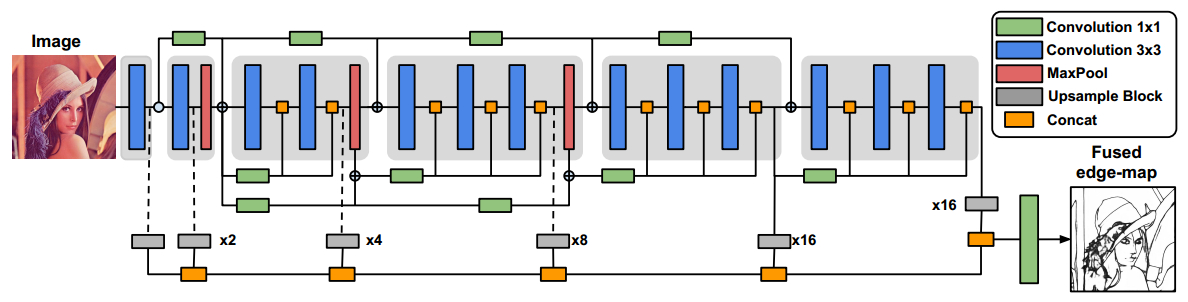
\includegraphics[width=\columnwidth]{picture/Edge Detection/DeixNed Architecture}
				\captionsetup{font=scriptsize}
				\caption{
					\label{fig: DeixNed Architecture} 
					 Proposed architecture: Dense Extreme Inception Network, consists of an encoder composed by six main blocks (showed in light gray). The main blocks are connected between them through 1x1 convolutional blocks. Each of the main blocks is composed by sub-blocks that are densely interconnected by the output of the previous main block. The output from each of the main blocks is fed to an upsampling block that produces an intermediate edge-map in order to build a Scale Space Volume, which is used to compose a final fused edge-map.
				}
			\end{figure}
		
			Fig. \ref{fig: DeixNed Architecture} 为 DexiNet 的网络架构,主要包含两个模块,一个是 Dexi 网络,一个是上采样模块 (灰色部分),RBG 图像输入 Dexi 网络进行特征提取 (Dexi网络能够较好的避免边缘信息的丢失),然后提取得到的特征图输入上采样模块进行边缘图像的生成,最后再将特征图进行融合,生成最终的边缘信息图像。
			
			\begin{figure}[htbp]
				% read manual to see what [ht] means and for other possible options
				\centering 
				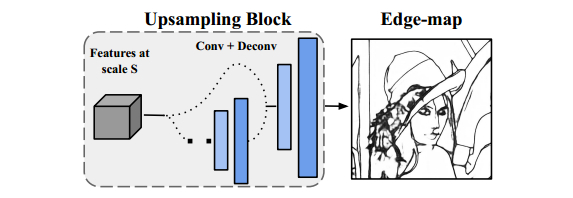
\includegraphics[width=0.7\columnwidth]{picture/Edge Detection/DeiXNed Upsampling Block}
				\captionsetup{font=scriptsize}
				\caption{
					\label{fig: DeixNed Architecture Block} 
					 Detail of the upsampling block that receives as input the learned features extracted from each of the main blocks. The features are fed into a stack of learned convolutional and transposed convolutional filters in order to extract an intermediate edge-map.
				}
			\end{figure}
			
			\subsubsection{Future}
			-
			
		\subsection{(2020.10) Deep Structural Contour Detection}
		
		\paragraph{深结构轮廓检测}
		
		\paragraph{(ACM MM 2020) doi: 10.1145/3394171.3413750}

			\subsubsection{Research Background}
			
			
			\subsubsection{Contribution}
			
			\begin{itemize}
				\item[(1)]
				作者提出了一种新颖且非常有效的轮廓检测损失函数。所提出的损失函数能够对每对预测与 GT 之间的轮廓结构相似性距离进行惩罚。
				
				\item[(2)]
				为了更好地区分目标轮廓和背景纹理,作者引入了一种新颖的卷积编码器-解码器网络。在网络中,作者提出了一个捕获高级特征之间密集连接并产生有效语义信息的超级模块。
			\end{itemize}
			
			\subsubsection{Approach}
			
			作者依照 LPCB, CED, RCF, HED
			
			\begin{figure}[htbp]
				% read manual to see what [ht] means and for other possible options
				\centering 
				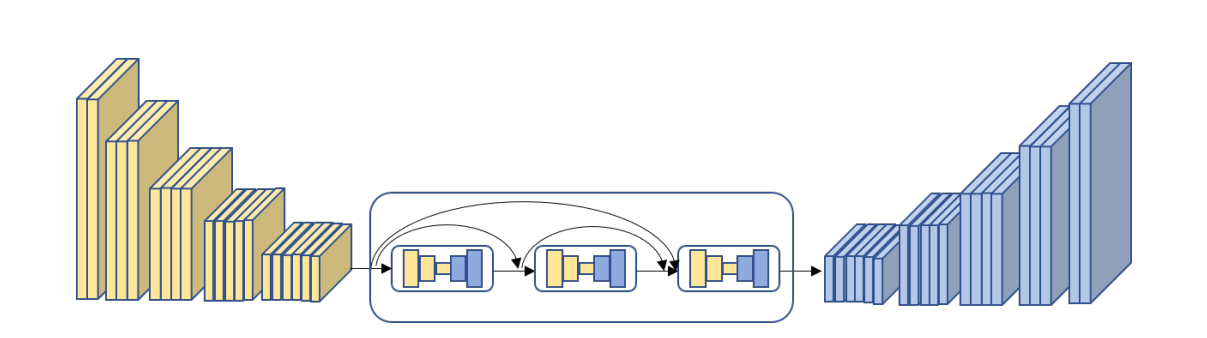
\includegraphics[width=\columnwidth]{picture/Edge Detection/DSCD proposed network}
				\captionsetup{font=scriptsize}
				\caption{
					\label{fig: DSCD proposed network} 
					Illustration of the proposed network. The left and the right are the encoder and the decoder, respectively. We adopt
					the VGG16 as our encoder. The encoder extracts multi-scale, multi-level features and the decoder fuse the features and recover the feature resolution to the original. The middle rectangle is the proposed hyper convolutional module. It adopts three conv blocks and captures dense connection among the hierarchical features. The module can significantly improve model
					performance. To the best view, we omit the connections between the encoder features and the decoder features.
				}
			\end{figure}
			
			
			\subsubsection{Future}
			-
		
		\renewcommand{\refname}{References}
		
		
		%	\begin{thebibliography}{00}
			
			%		\bibitem{b1}\label{cite:b1}
			%		W. Wang, C. Wei, W. Yang and J. Liu, "GLADNet: Low-Light Enhancement Network with Global Awareness," 2018 13th IEEE International Conference on Automatic Face \& Gesture Recognition (FG 2018), Xi'an, China, 2018, pp. 751-755, DOI: 10.1109/FG.2018.00118.
			
			%		\bibitem{b2}\label{cite:b2}
			%		A.\ Mahajan, K.\ Somaraj and M. Sameer, "Adopting Artificial Intelligence Powered ConvNet To Detect Epileptic Seizures," 2020 IEEE-EMBS Conference on Biomedical Engineering and Sciences (IECBES), Langkawi Island, Malaysia, 2021, pp. 427-432, DOI: 10.1109/IECBES48179.2021.9398832.
			
			%		\bibitem{Cyr}
			%		N.\ Cyr, M.\ T$\hat{e}$tu, and M.\ Breton,
			% "All-optical microwave frequency standard: a proposal,"
			%		IEEE Trans.\ Instrum.\ Meas.\ \textbf{42}, 640 (1993).
			
			
			
			%	\end{thebibliography}
		
		\bibliographystyle{unsrt}
		\bibliography{reference}
		
		
	\end{document}
